%\vspace{-1.5em}
\section{Introduction}
%\vspace{-1em}
Object manipulation remains a core challenge for robot learning, but the factors that make it difficult to learn generalist manipulation policies remain unclear. Most existing approaches rely heavily on either expert demonstrations~\citep{vecerik2017leveraging, zitkovich2023rt, kim2024openvla, chi2025visuomotor, o2024open} or carefully designed reward functions~\citep{ma2024eureka, tang2025deep}. While these paradigms have impressive progress, they also introduce strong supervision requirements:  demonstrations can be expensive to collect and may cover only a narrow range of behaviors, while task-specific rewards often require substantial engineering and do not easily scale to open-ended multitask settings. These limitations motivate unsupervised approaches that can acquire reusable manipulation skills and representations directly from interaction, without assuming demonstrations or manually specified rewards~\citep{eysenbach2018diversity, touati2021learning, laskin2022unsupervised, park2024metra, agarwal2025unified}. Among them, goal-conditioned Reinforcement Learning (GCRL) offers a promising direction for learning a family of policies to handle the inherent multitask nature of manipulation~\citep{liu2022goal}. Successful GCRL requires learning strong representations to capture the shared properties between different control behaviors. While the strategies for learning these representations remain an open challenge, recent work in Contrastive Reinforcement Learning (CRL) offers a promising direction forward~\citep{eysenbach2022contrastive}. CRL has shown impressive capabilities to learn complex control from scratch, and even limited success in manipulation tasks~\citep{liu2025single}. However, despite the clear fit of GCRL algorithms for manipulation, their performance remains limited.


%In this work, we ask a central question: \textit{when and why does CRL fail for manipulation}, and \textit{what is needed to make it work}? We identify \textit{interactions} as a core property of manipulation that makes effective policy representation difficult. Specifically, these relational events between entities induce distinct changes in dynamic modes. 
%These induced mode changes make the CRL representation no longer well approximated by the linear-Gaussian structure observed in locomotion tasks~\citep{eysenbach2024inference}, thereby making planning over this representation space substantially more difficult. To formalize this challenge, we view manipulation as a mode-switching dynamical system, where the active mode changes across phases before, during, and after an interaction. These interaction-dependent modes induce piecewise nonlinear dynamics that are substantially harder to represent than the smoother structures often observed in locomotion tasks. This provides a concrete mechanism for why CRL representations can become poorly shaped in manipulation: they may smooth over critical interaction boundaries and fail to capture the mode changes that determine future reachability. We empirically observe this failure mode and show how it leads to poor policy performance, as illustrated in Figure~\ref{fig:intro_energy}.

In this work, we ask a central question: \textit{when and why does CRL fail for manipulation}, and \textit{what is needed to make it work}? We identify \textit{interactions} as a core property of manipulation that makes effective policy representation difficult. Specifically, interactions are relational events between entities that induce distinct changes in dynamic modes. Since CRL relies on the learned representation to define goal-reaching energies for planning, these interaction-induced mode changes can substantially distort the geometry over which policies are learned and planned.

To formalize this challenge, we view manipulation as a mode-switching dynamical system, where the active mode changes across phases before, during, and after an interaction. These interaction-dependent modes induce piecewise nonlinear dynamics and reachability structures that are substantially harder to represent than the smoother structures often observed in locomotion tasks, which can be well approximated by linear-Gaussian dynamics~\citep{eysenbach2024inference}. This provides a concrete mechanism for why CRL representations can become poorly shaped in manipulation: they may smooth over critical interaction boundaries and fail to capture the mode changes that determine future reachability. We empirically observe this failure mode and show how it leads to poor policy performance in Fig.~\ref{fig:example}.
\begin{wrapfigure}{r}{0.48\textwidth}
    \centering
    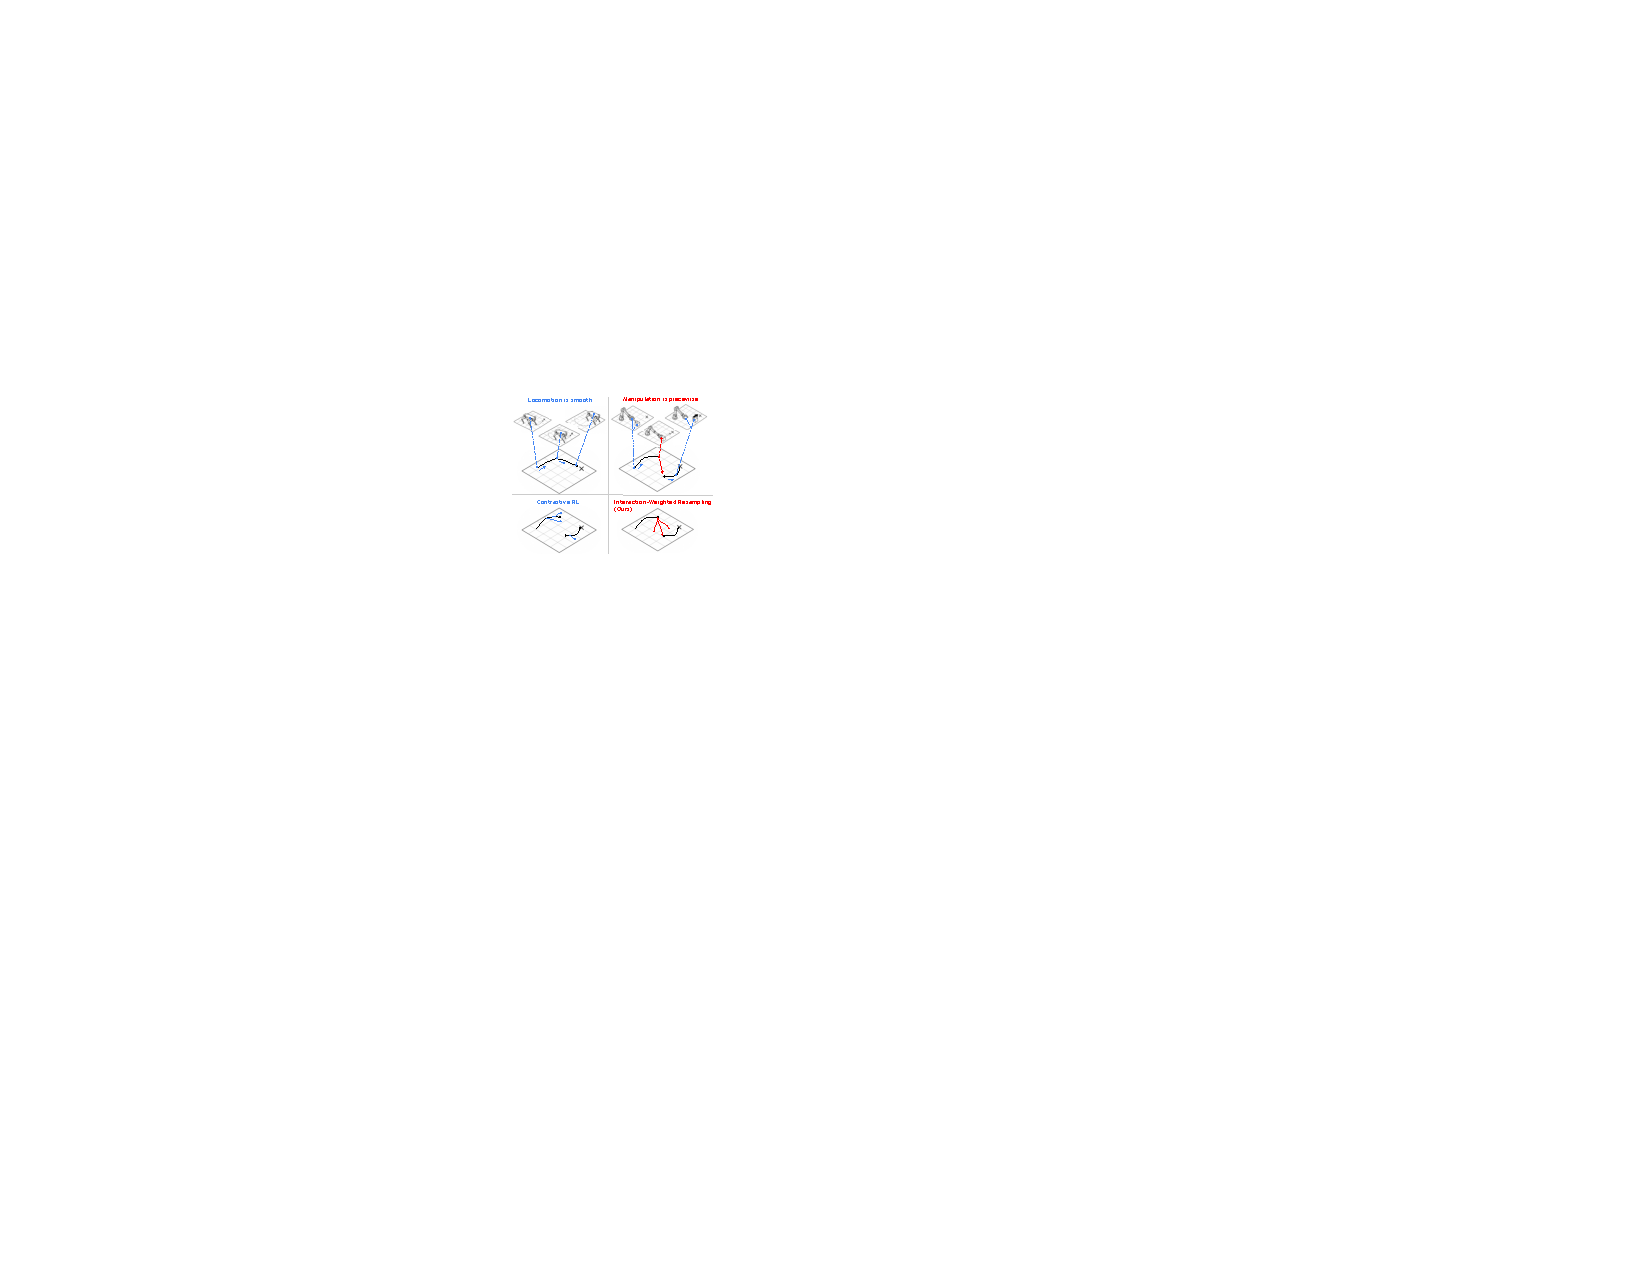
\includegraphics[width=0.47\textwidth]{figure/example-fig-1.pdf}
    \caption{\textbf{Motivation}. In locomotion-like domains, future reachability often follows a smooth temporal structure, making standard CRL effective.  In manipulation, object interactions induce piecewise mode changes, causing standard CRL to miss critical interaction transitions.  IWR  emphasizes these interaction-relevant points to better learn the goal-reaching energy.
}    
\label{fig:example}    
\vspace{-15pt}
\end{wrapfigure}
%Formally, we model this challenge in manipulation as changes in dynamic modes---before, during and after an interaction. Unlike more amenable tasks like locomotion, these modes induce piecewise nonlinearities that are significantly more difficult to model. In fact, we empirically observe these limitations and how they induce poor performance, which we illustrate in Figure~\ref{fig:intro_energy}. 

%Interactions form one of the core challenges for manipulation by forcing models of the dynamics to handle non-smooth, exponentially variable futures. These futures are especially difficult to learn, and without a careful treatment of these dynamics, can often render manipulation tasks infeasible~\citep{}. We formalize the challenges of interactions in manipulation as changes in dynamic modes---before, during and after an interaction. Unlike more amenable tasks like locomotion, these modes induce piecewise nonlinearities that are significantly more difficult to model, even for representation learning algorithms such as CRL. In fact, we empirically observe these limitations and how they induce poor performance, which we illustrate in Figure~\ref{fig:intro_energy}

%Interactions form one of the core challenges for manipulation by forcing models of the dynamics to handle non-smooth, exponentially variable futures. These futures are especially difficult to learn, and without a careful treatment of these dynamics, can often render manipulation tasks infeasible~\citep{}. 

%By understanding provably interactions as a core challenge of manipulation, we propose a straightforward scheme to improve the learning of these piecewise non-linearities through two insights:
Guided by our analysis of how interactions induce piecewise nonlinear structure in manipulation, we propose a principled yet simple scheme to improve CRL in these settings. Building on insights from interaction modeling~\citep{chuck2023granger, hwang2024fine, chuck2025null, lei2026spartan} and combinatorial resampling~\citep{kim2024enhancing, ziarko2026contrastive}, we introduce \methodname{} (\methodshort{}), a contrastive resampling principle that reshapes the training distribution toward interaction-induced mode transitions. Instead of treating all transitions uniformly, \methodshort{} constructs informative state-goal comparisons around interaction-relevant points, encouraging the representation to preserve the mode boundaries that govern future reachability. 
Through evaluation on robotic manipulation domains with complex object interactions, including Meta-World, simulated dynamic maze environments, and robot air hockey, we show that \methodshort{} provides a principled way to address the core challenges of CRL by improving both its training distribution and representation capacity. \methodshort{} achieves significantly better sample efficiency and overall performance than prior GCRL methods. Notably, we demonstrate the first goal-conditioned robot air hockey agent capable of hitting multiple goals from a dynamically moving puck.

%Our approach is based on two key insights: \textbf{1)} Combining prior work related to interaction~\citep{} and combinatorial resampling~\citep{}, we introduce \methodname{}, which directs the representations to emphasize interaction-relevant points. \textbf{2)} By recognizing the challenge of learning a representation that can handle multiple modes, we introduce \archname{,} a network augmentation that allows the model to capture greater complexity in how the future distribution can be reached from the current distribution, including nonlinear relationships. We demonstrate that these two modifications are principled solutions to the core challenge by modeling the distribution and representation capacity of CRL. Combining \methodname{} and \archname{}, we are able to demonstrate significantly improved sample efficiency and overall performance compared to prior GCRL work in interaction-centric environments, including: dynamic maze domains, robotic manipulation, and robot air hockey, demonstrating the first instance of a goal-conditioned robot air hockey agent that can hit multiple goals from a dynamically moving puck. 

%In summary, our contributions are:
%\begin{enumerate}
%    \item Formalizing the core challenge of representation learning for robot manipulation with interactions
%    \item Introducing \methodname{} and \archname{} to address these challenges, and empirically validating their effectiveness.
%    \item Providing proofs for the theoretical properties of the interaction weighting
%\end{enumerate}

Our contributions are: \textbf{\textit{(i)}} a principled analysis of why interaction-rich manipulation poses a fundamental challenge for CRL
% , showing how interaction-induced mode changes lead to piecewise nonlinear reachability structures that are difficult to represent and plan over; 
\textbf{\textit{(ii)}} Introducing \methodname{} (\methodshort{}), inspired by this principled analysis, which reshapes the effective contrastive training distribution toward interaction-relevant transitions.
% to capture multi-modal, piecewise nonlinear reachability; 
\textbf{\textit{(iii)}} Empirical validation of \methodshort{}
% , showing how it improves the learning of interaction-relevant representations, and empirically validate our method 
across dynamic maze domains, robotic manipulation, and substantial improvement in robot air hockey.
